%----------------------------------------------------------------------------
\chapter{Test design}
%----------------------------------------------------------------------------
\section{Test approaches}
The railway demonstrator system is a multi-layered application, which models a safety critical railway system. In that manner we have to make sure that we detect all the failures during the design and development phase. For this purpose in the following section I will investigate the test opportunities for the MoDeS$^3$ system.

\begin{figure}[h]
	\centering
	\includegraphics[width=150mm]{figures/modes3/v_model.png}
	\caption{V-model}
	\label{fig:vModel}
\end{figure}

\paragraph{V-model and testing levels}
Nowdays one of the most popular software development methodology is the V-model (on figure \ref{fig:vModel}), which defines four stages during the development and four verification steps accordingly (shown with rectangles). In addition for making the development more effective for error-detection, there are three more steps for verifying our system (shown with ellipses). While the development starts with an abstract \textbf{requirement analysis} which declares the aim of our application, later on each step contains more detailed information. The second phase is about understanding the abstract user requirements and define the \textbf{system functional specification} by the developers. During this phase our verification is based on \textbf{Model-in-the-Loop (MiL) testing}. The third phase contains all the low-level design and specific information about the application. From these design decisions, the \textbf{implementation} should be quite straight-forward or even generated. To make sure that the code is working correctly it is tested using \textbf{Software-in-the-Loop (SiL)}. 
As of now our application code is written and our design decisions are verified, we make sure with \textbf{unit tests} that our functions are working well on their own. \textbf{Processor-in-the-Loop (PiL)} testing can be made here. Moving up in the V-model with \textbf{integration tests}, we are focusing on more abstract and complex components. In this phase we consider software and hardware elements also, completed with \textbf{Hardware-in-the-Loop (HiL)} testing. The last step is about verifying the complete system in real environment and check the high-level criterias.

\section{Test scenarios}
In the following section I will examine the test opportunities for the MoDeS$^3$ system.  The \ref{table:test_cases} table shows the software components for different test levels. In the table a checkmark shows the possibility to test that component in that exact level. For the other cases testing is irrelevant. I have defined four integration test layouts, and for each test layout a component is involved where a checkmark is shown. All the software components, which is deployed to other hardware components have network communication, therefore the messenger software component is involved in the test.

In addition not all the software component have been mentioned  on the \ref{table:test_cases} table, because not safety critical components have been skipped. Barrier is irrelevant regarding the train-collision detection. How the trains get speed and direction controls is not safety critical either, so LeapMotion and XPressNet components are not safety critical. Touchboard and Dashboard components are visualising the railway current states send commands to the system, so not relevant elements in terms of train collision.

\begin{table}[h]
	\caption{Component test possibilities in test levels}
	\label{table:test_cases}
	\begin{center}
		\renewcommand{\arraystretch}{1.5}
		\begin{tabu} 
			to 0.9 \textwidth
			 {  m{4.5 cm}  c  X[c] X[c] X[c] X[c]  X[c]  }
			\toprule
			\centeredDoubleRow{2}{Component Name} & \centeredDoubleRow{2}{Component} &          \multicolumn{4}{c}{Integration}          & System     \\
			\cmidrule(rl){3-6} \cmidrule(l){7-7}  &                                  & layout 1   & layout 2   & layout 3   & layout 4   & layout 1   \\ \midrule
			Section Occupancy Query               & \checkmark                       & \checkmark &            & \checkmark &            & \checkmark \\
			Occupancy Query                       & \checkmark                       & \checkmark &            & \checkmark &            & \checkmark \\
			GPIO                                  & \checkmark                       &            & \checkmark &            & \checkmark & \checkmark \\
			Track Element Controller              & \checkmark                       &            & \checkmark &            & \checkmark & \checkmark \\
			Safety Logic                          & \checkmark                       &            &            & \checkmark & \checkmark & \checkmark \\
			Messenger                             &                                  & \checkmark &            & \checkmark & \checkmark & \checkmark \\ \bottomrule
		\end{tabu}
	\end{center}
\end{table} 

\todo[inline]{Figure of affected components of the layout (sysml with rectangles)}
\paragraph{Integration test layout 1}
Aim of this test case is the occupancy detection, which functional operation is described in \ref{section:OccupancyDetection} section. One track element is occupied if a train is moving or stopped on the element. In hardware point of view this detection is made by the DigiSens-8-S88 sensor, which is an off-the-shelf product, so we do not want to test it.  

\paragraph{Integration test layout 2}
Aim of this test is to verify the software components, which is deployed to the BBB (described in \ref{par:FunctionTEC} section) and responsible for controlling the physical segments. All the 6 BBB have separate instance of \textbf{Track Element Controller}. This component gets and information through the network on command topics, when segment granting or turnout state must be changed. At this point the control differentiates into subcomponents weather a turnout or a section command have been received. Both branches use GPIO software component for giving impulse on the BBB cape pins. 

\paragraph{Integration test layout 3}
In this integration test a more complex strategy comes into picture. After we have verified the \textbf{Safety Logic} and the occupancy detection elements, we can investigate the \textbf{Safety Logic} decision based on the generated occupancy states. These signs can be injected into the \textbf{Arduino} hardware element or into the Section Occupancy Query directly.

\paragraph{Integration test layout 4}
The fourth integration test should verify the action after a \textbf{Safety Logic} decision. In details, we can inject a critical scenario into the \textbf{Safety Logic} component where a safety intervention needed, and check the GPIO component's file writing operation.

\paragraph{System Test}
In the system tests all component is involved, and only the injected scenario is different. 
I have already mentioned a few collision scenario in \ref{par:trainScenarios} section, and I just one to add three more scenarios with the double-turnout. The first layout (see figure \ref{fig:LayoutT3-scenario1}) is a typical case, where the collision can be easily avoided with \textit{Train 1} waiting.
\begin{figure}[!h]
	\centering
	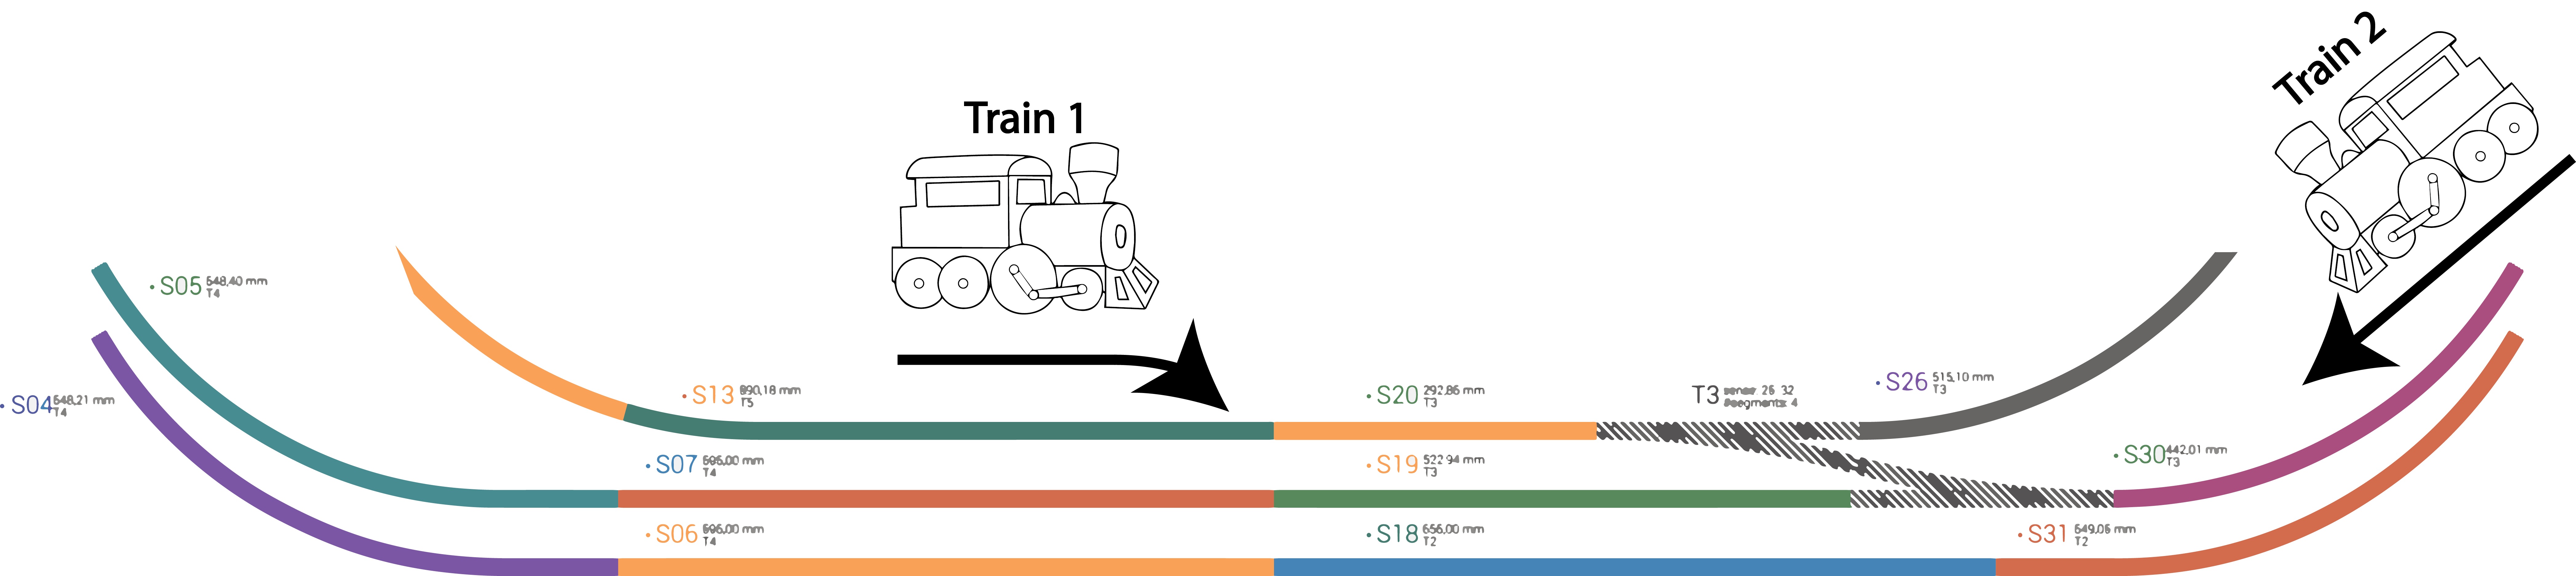
\includegraphics[width=150mm, keepaspectratio]{figures/modes3/layoutT3-scenario1.png}
	\caption{Turnout 3 collision scenario 1}
	\label{fig:LayoutT3-scenario1}
\end{figure}
The next possible collision could happen, when our two trains going exactly into each other after 2 sections.
\begin{figure}[!h]
	\centering
	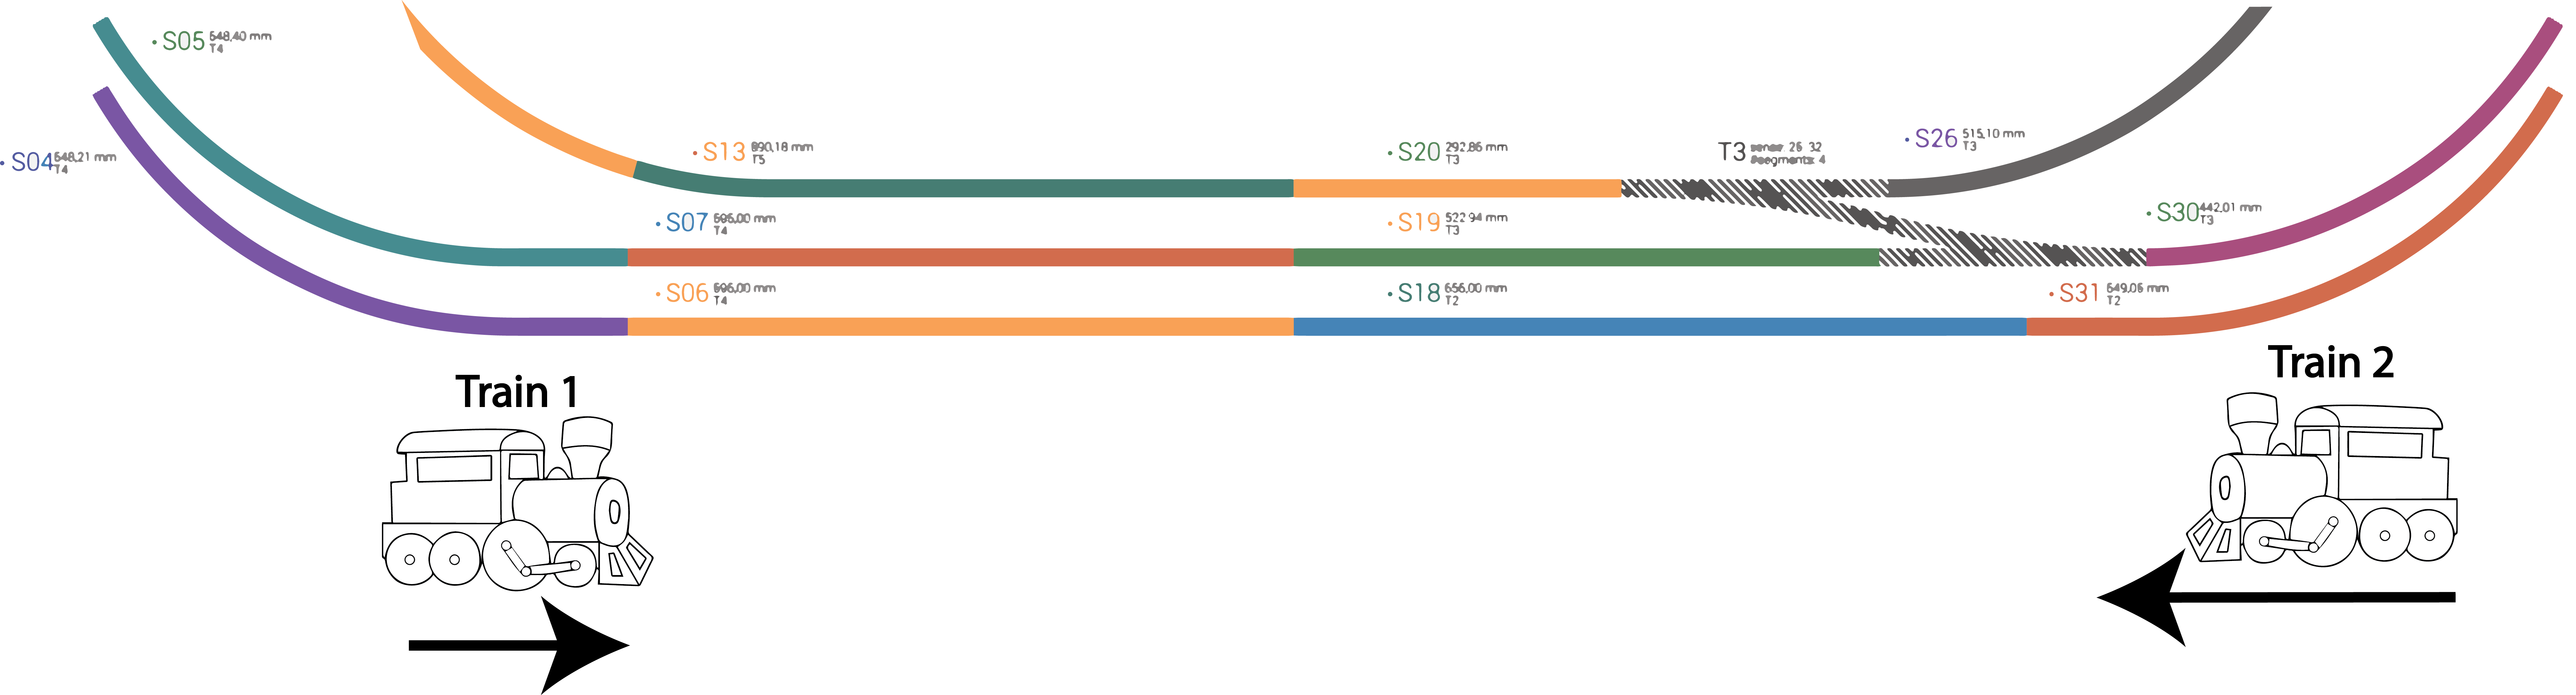
\includegraphics[width=150mm, keepaspectratio]{figures/modes3/layoutT3-scenario2.png}
	\caption{Turnout 3 collision scenario 2}
	\label{fig:LayoutT3-scenario2}
\end{figure}
The third scenario is similar with the first one, but if our T3 turnout is in a right direction (both turnout is in the straight direction), our trains are safe.
\begin{figure}[!h]
	\centering
	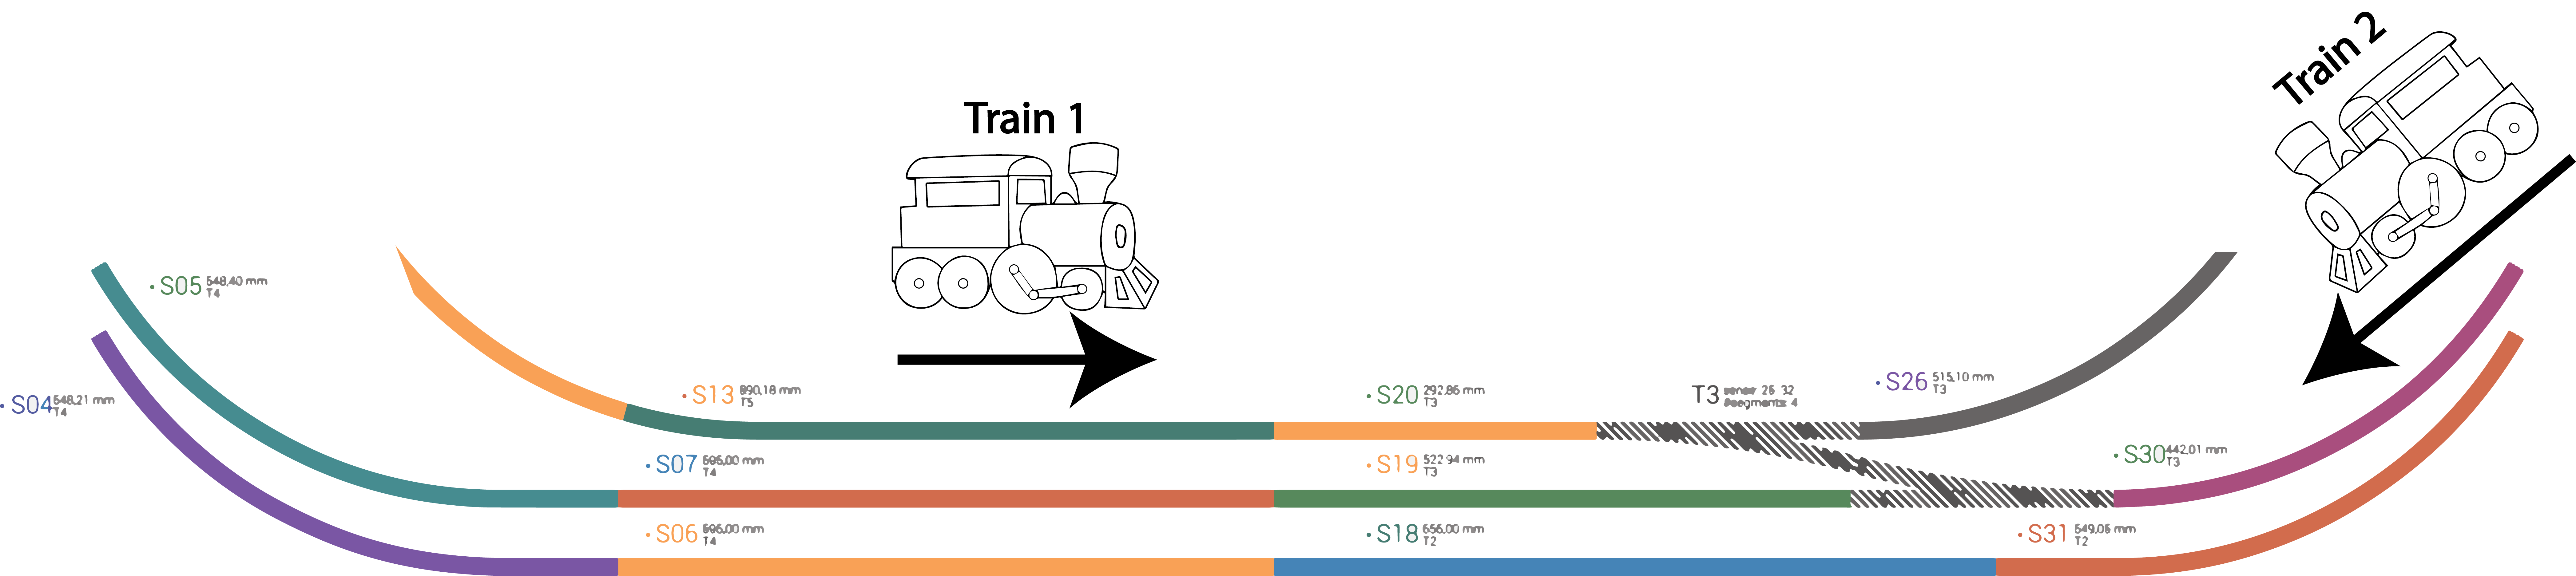
\includegraphics[width=150mm, keepaspectratio]{figures/modes3/layoutT3-scenario3.png}
	\caption{Turnout 3 collision scenario 3}
	\label{fig:LayoutT3-scenario3}
\end{figure}